\documentclass[a4paper,english,tikz]{report}

\usepackage{graphicx}
\usepackage{float}
\usepackage[parfill]{parskip}
\usepackage[T1]{fontenc}
\usepackage{textcomp}
\usepackage{markdown}
\usepackage{minted}
\usepackage{tcolorbox}
\usepackage{etoolbox}
\usepackage[edges]{forest}
\usepackage{multicol}
\usepackage{graphics}
\usepackage{enumitem}
\usepackage[ampersand]{easylist}
\usepackage[utf8]{inputenc}
\usepackage[english]{babel}
\usepackage{hyperref}

% table package
% \usepackage[table]{xcolor}
\usepackage{array}
\usepackage{tabularx}
\usepackage{multirow}
\usepackage{longtable}

% no indent
\setlength{\parindent}{0pt}

% setup list
\setlist[itemize]{leftmargin=*}

% setup forest
\usetikzlibrary{shadows,arrows.meta}

% setup minted
\usemintedstyle{emacs}
% {frame=lines,framerule=2pt}
% {frame=single,framesep=2pt}
\setminted{breaklines}
\setmintedinline{breaklines} % necessary for breakanywhere to work later on.

% \BeforeBeginEnvironment{minted}{\begin{tcolorbox}}%
% \AfterEndEnvironment{minted}{\end{tcolorbox}}%

\newcommand{\cppinline}[1]{\mintinline{cpp}{#1}}

% setup multicols
\setlength{\columnsep}{1cm}

% setup links
\hypersetup{
  colorlinks=true,
  linkcolor=blue,
  filecolor=magenta,
  urlcolor=cyan,
  pdftitle={rayandrew's research},
  bookmarks=true,
  pdfpagemode=FullScreen,
}

% setup subsection
\usepackage{titlesec}
\titleclass{\subsubsubsection}{straight}[\subsection]

\newcounter{subsubsubsection}[subsubsection]
\renewcommand\thesubsubsubsection{\thesubsubsection.\arabic{subsubsubsection}}
\renewcommand\theparagraph{\thesubsubsubsection.\arabic{paragraph}} % optional; useful if paragraphs are to be numbered

\titleformat{\subsubsubsection}
{\normalfont\normalsize\bfseries}{\thesubsubsubsection}{1em}{}

\titlespacing*{\subsubsubsection}
{0pt}{3.25ex plus 1ex minus .2ex}{1.5ex plus .2ex}

\makeatletter
\renewcommand\paragraph{\@startsection{paragraph}{5}{\z@}%
  {3.25ex \@plus1ex \@minus.2ex}%
  {-1em}%
  {\normalfont\normalsize\bfseries}}
\renewcommand\subparagraph{\@startsection{subparagraph}{6}{\parindent}%
  {3.25ex \@plus1ex \@minus .2ex}%
  {-1em}%
  {\normalfont\normalsize\bfseries}}
\def\toclevel@subsubsubsection{4}
\def\toclevel@paragraph{5}
\def\toclevel@paragraph{6}
\def\l@subsubsubsection{\@dottedtocline{4}{7em}{4em}}
\def\l@paragraph{\@dottedtocline{5}{10em}{5em}}
\def\l@subparagraph{\@dottedtocline{6}{14em}{6em}}
\makeatother

\setcounter{secnumdepth}{4}
\setcounter{tocdepth}{4}

\begin{document}

\title{UCARE Research}
\author{Ray Andrew}

\maketitle

\begin{abstract}
The abstract text goes here.
\end{abstract}

\tableofcontents
\newpage

\section{Todos}

\subsection{03 November 2019}
\begin{itemize}
\item Add markOop memory layout
\item Upload docs into github
\item Test dedup System.copyarray 
\end{itemize}

\newpage

\section{Meeting Notes}

\subsubsection{09 October 2019}

\begin{itemize}
\item Try the Kafka sytem inside Eclipse OpenJ9 test whether parameter classdatashare is working or not
\item IBM Java Multitenancy
\item See implementation of native function (arrayCopy) and try see how the copy the array and look into the content
\item No matplotlib and try to change it GNUPlot
\end{itemize}
\subsubsection{22 October 2019}

\begin{itemize}
\item Create our own SLABs, 32 Nodes, 7 Workloads
\item Check if object is unmodified
\item Understand what is Klass, MarkOop, Array looks like on memory layout
\item send me string dedup paper, read it and we discuss it next tuesday
\end{itemize}
\subsubsection{30 October 2019}

\begin{itemize}
\item 1 more week to implement arraycopy to check whether we can call slab allocation directly (basically mmap)
\item Mark class memory layout
\item Upload the documents
\item Check implementation of String Deduplication in OpenJ9
\item Continuing other bugs
\end{itemize}
\subsubsection{05 November 2019}

\begin{itemize}
\item Using jmap to dump the JVM, see this link : \href{https://stackoverflow.com/questions/32605962/locate-and-read-objects-of-a-specific-type-from-memory-of-a-running-java-program}{Jmap}
\item do sample program to allocate one array of ints (size 10) and run into two or three JVMs, dump that array
\item check what is different, what is the same
\item differences in object layout
\end{itemize}
\subsubsection{17 December 2019}

\begin{itemize}
\item Write why those KSM works (a summary) (1-2 pages)
\end{itemize}
\subsubsection{07 January 2020}

% - 1 instance of systems -> running a workload -> we need to know at some point X objects
% - and at Y systems -> how many objects ?
% - what is the intersection between X and Y

% e.q =
% - 2 running replicas run workloads -> how many objects that have the same data?

% - we need to know how these 2 objects are equivalent?

% ideas :
% - we need a notion of equivalence
% - we need to apply this notion to all objects

% steps :
% - using JVMTI in the callbacks -> to iterate all objects in Heap
% - for each one of objects we will try to compare to another JVMs
% - we want to check the objects between two objects
% - given two instances -> looking at the content -> are they same?

\begin{itemize}
\item we only share `all pages` not the `real data`
\item how can we be more specific -> to save the real data instead of whole heap?
\item we need to go deeper into `old generation` itself and find the real content
\item questions
  \begin{itemize}
  \item 1 instance of systems -> running a workload -> we need to know at some point X objects
  \item and at Y systems -> how many objects?
  \item what is the intersection between X and Y
  \item e.q =
  \item 2 running replicas run workloads -> how many objects that have the same data?
  \end{itemize}

\item steps
  \begin{itemize}
  \item using JVMTI in the callbacks -> to iterate all objects in Heap
  \item for each one of objects we will try to compare to another JVMs
  \item we want to check the objects between two objects
  \item given two instances -> looking at the content -> are they same?
  \end{itemize}
\end{itemize}
\newpage

\section{Summaries}

\subsection{Memory Deduplication}
\subsubsection{Introduction}

\subsubsubsection{Virtualization}

Virtualization is used throughout the world and one of growing trend for hosting services within data-centers. \cite{rachamalla_mishra_kulkarni_2013}
Virtualization uses dynamic resource allocation and migration techniques. Memory over-commit is one of commonly used technique to facilitate server consolidation where the total memory size for all running VMs exceeds actual pyshical memory of hypervisor.

\textbf{There are two improvements that have been done to overcome this issue:}
\begin{enumerate}
\item Demand paging -> pages are swapped back and forth to alleviate memory requirements of VMs
\item Memory ballooning -> inflated to force the machine to relinquish pages according to it's local memory management policy
\item Exploit redundancy of memory content
\end{enumerate}

\subsubsubsection{Content Based Page Sharing (CPBS)}

One of major feature that has been implemented throughout hypervisors around the world.
Another essential feature of \textbf{CPBS} is \textbf{CPBS} able to perform transparently in the hypervisor layer and doesn't require any modification to guest OS / process.

\textbf{Classified into two categories:}
\begin{enumerate}
\item in-band sharing -> same page detection and merging in the I/O path (mostly disk access path)
\item out-band sharing -> periodically scans memory to identify and merge shareable pages
\end{enumerate}

Out-of-band sharing techniques can potientially take advantage of complete system memory to identify identical memory pages. Out-of-band techniques such as KSM, usually \textbf{oscillate between a sleep period and a scan period}
\subsubsection{Kernel Samepage Merging (KSM)}

\subsubsubsection{Introduction}
Created by RedHat, Inc. in this paper \cite{arcangeli_andrea_edius_ksm_2009}
in team consists of Andrea Arcangeli, Izik Eidus, Chris Wright.

\textbf{The main goal is to:} share equal anonymous memory across different processes and in turn also across different KVM virtual machines.

One thing to remember is: \textbf{KSM is not only for KVM virtual machines, all processes that has equal anonymous memory can be shared through KSM daemon}

\subsubsubsection{Algorithm}

\textbf{KSM daemon uses two  global red-black comparisons tree for whole memory pages:}
\begin{enumerate}
\item \textbf{Stable tree} contains already shared pages with write-protected
\item \textbf{Unstable tree} contains only pages that are not shared yet but tracked with KSM (without write-protected)
\end{enumerate}

To reduce the number of false negative from the unstable tree lookups, a checksum is used to insert into the unstable tree only pages whose checksum didn’t change recently.

\textbf{KSM deduplication process:}
\begin{enumerate}
\item Calculate checksum of page and compare to its last checksum
  \begin{itemize}
  \item if match : become candidate page, continue to compare page with pages in stable trees
  \item else     : volatile page
  \end{itemize}
\item *Every* candidate page is compared with pages in stable tree
  \begin{itemize}
  \item if match : candidate page will be merged and shared with matched KSM page -> end
  \item else     : search to unstable tree
  \end{itemize}
\item *Every* candidate page is compared with pages in unstable tree
  \begin{itemize}
  \item if match : matched page will be removed from unstable tree and merged to stable tree with write-protected
  \item else     : candidate page is inserted into the unstable tree (as leaf node)
  \end{itemize}
\item Each scan, unstable tree needs to be reconstructed to get correct node position. this must be done because of pages in unstable tree are not write-protected -> content might be modified during the scan round
\item If multiple pages with same content are detected, one of pages is selected as KSM page, and merge other duplicate pages
\item Original space of duplicate pages are reclaimed and saved
\end{enumerate}

\textbf{Charts:}
Can be seen through this figure below

\begin{figure}[H]
  \centering
  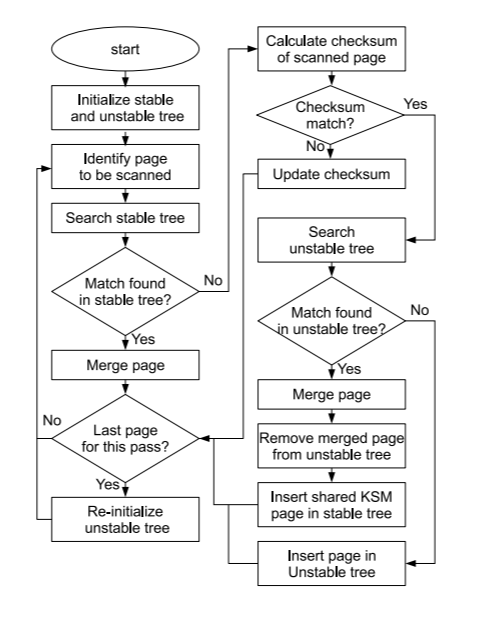
\includegraphics[width=\linewidth]{_summaries/deduplication/_images/ksm-algo.png}
  \caption{KSM Algorithm}
  \label{fig:ksm1}
\end{figure}

\subsubsubsection{API}
KSM is a Linux kernel thread that run independently on demand when virtual areas is registered as mergeable.

\begin{minted}{cpp}
#include <sys/mman.h>

int madvise(void *addr, size_t length, int advice);
\end{minted}

\textbf{int advice:}
\begin{itemize}
\item \textbf{MADV\_MERGEABLE} (since Linux 2.6.32) \\
  Enable Kernel Samepage Merging (KSM) for the pages in the
  range specified by addr and length.  The kernel regularly
  scans those areas of user memory that have been marked as
  mergeable, looking for pages with identical content.  These
  are replaced by a single write-protected page (which is
  automatically copied if a process later wants to update the
  content of the page).  KSM merges only private anonymous pages
  (see mmap(2)).
  
  The KSM feature is intended for applications that generate
  many instances of the same data (e.g., virtualization systems
  such as KVM).  It can consume a lot of processing power; use
  with care.  See the Linux kernel source file
  Documentation/admin-guide/mm/ksm.rst for more details.

  The \textbf{MADV\_MERGEABLE} and \textbf{MADV\_UNMERGEABLE} operations are
  available only if the kernel was configured with \textbf{CONFIG\_KSM}.

\item \textbf{MADV\_UNMERGEABLE} (since Linux 2.6.32) \\
  Undo the effect of an earlier \textbf{MADV\_MERGEABLE} operation on the
  specified address range; KSM unmerges whatever pages it had
  merged in the address range specified by addr and length.
\end{itemize}

\vspace{5mm}

\textbf{Caveats:}
\begin{itemize}
\item KSM is possible to scan all anonymous page but it should be wasteful where we cannot find equal anonymous pages.

\item To keep track of the pages, KSM uses \textbf{Slab Allocation}. \\ The number of slab allocation is linearly increasing with the size of registered virtual areas.
\end{itemize}

\vspace{5mm}

\textbf{The KSM behavior can be controlled through sysfs at /sys/kernel/mm/ksm/:}
\begin{itemize}
\item \textbf{run}
  \begin{itemize}
  \item 1 for running
  \item 0 for stop
  \item 2 for stop ksmd and unmerge all pages currently merged, but leave mergeable areas registered for next run
  \end{itemize}
\item \textbf{pages\_to\_scan} -> how many pages to scan before ksmd go to sleep, e.g. 100
\item \textbf{sleep\_millisecs} -> how many milliseconds ksmd should sleep before next scan, e.g. 20
\item \textbf{merge\_across\_nodes} -> specifies if pages from different NUMA nodes can be merged
  \begin{itemize}
  \item 0 -> ksm merges only pages which physically reside in the memory area of same NUMA node. That brings lower latency to access of shared pages. Systems with more nodes, at significant NUMA distances, are likely to benefit from the lower latency
  \item 1 (default) -> Smaller systems, which need to minimize memory usage, are likely to benefit from the greater sharing
  \end{itemize}
\item \textbf{use\_zero\_pages} -> specifies whether empty pages (i.e. allocated pages that only contain zeroes) should be treated specially
  \begin{itemize}
  \item 0, normal behavior
  \item 1, empty pages are merged with the kernel zero page(s) instead of with each other as it would happen normally. This can improve the performance on architectures with coloured zero pages, depending on the workload. Care should be taken when enabling this setting, as it can potentially degrade the performance of KSM for some workloads, for example if the checksums of pages candidate for merging match the checksum of an empty page
  \end{itemize}
\item \textbf{max\_page\_sharing} -> Maximum sharing allowed for each KSM page, to avoid high latency for virtual memory operations that involve traversal of virtual mappings that share the KSM page
\item \textbf{stable\_node\_chains\_prune\_millisecs} -> specifies how frequently KSM checks the metadata of the pages that hit the deduplication limit for stale information
\end{itemize}

\vspace{5mm}

\textbf{The KSM effectiveness can be seen through sysfs at /sys/kernel/mm/ksm/ with this parameter:}
\begin{itemize}
\item \textbf{pages\_shared} -> how many shared pages are being used
\item \textbf{pages\_sharing} -> how many more sites are sharing them i.e. how much saved
\item \textbf{pages\_unshared} -> how many pages unique but repeatedly checked for merging
\item \textbf{pages\_volatile} -> how many pages changing too fast to be placed in a tree
\item \textbf{full\_scans} -> how many times all mergeable areas have been scanned
\item \textbf{stable\_node\_chains} -> the number of KSM pages that hit the \textbf{max\_page\_sharing} limit
\item \textbf{stable\_node\_dups} -> number of duplicated KSM pages
\end{itemize}

\vspace{5mm}

\subsubsubsection{Sum up}
\begin{enumerate}
\item KSM is to increase memory density
\item KSM is generating shared pages by merging equal pages, and in turn it is making free memory available allowing to run more virtual machines or applications on the same system, than otherwise would be possible without KSM
\item A high ratio of \textbf{pages\_sharing} to \textbf{pages\_shared} indicates good sharing, but a high ratio of \textbf{pages\_unshared} to \textbf{pages\_sharing} indicates wasted effort. \textbf{pages\_volatile} embraces several different kinds of activity, but a high proportion there would also indicate poor use of madvise \textbf{MADV\_MERGEABLE}.
\end{enumerate}

\subsection{JVM Hotspot}
\subsubsection{Oop Hierarchy}
\label{summarization:jvm:oop_hierarchy}

\begin{center}
  \begin{minted}{cpp}
    typedef class oopDesc*                                  oop;
    typedef class   instanceOopDesc*                instanceOop;
    typedef class   arrayOopDesc*                      arrayOop;
    typedef class     objArrayOopDesc*              objArrayOop;
    typedef class     typeArrayOopDesc*            typeArrayOop;
  \end{minted}
\end{center}
\subsubsection{Oop Memory Layout}
\label{summarization:jvm:oop_memory_layout}

\begin{enumerate}

\item narrowKlass = int, sizeof = 4

\item \cppinline{const int HeapWordSize       = 8;}
\item \cppinline{const int LogBytesPerLong    = 3;}
\item \cppinline{const int BytesPerLong       = 1 << LogBytesPerLong;}
\item \cppinline{const int HeapWordsPerLong   = BytesPerLong / HeapWordSize;}

\item Instance Oops for Object
  \begin{center}
    \resizebox{\textwidth}{!}{%
      \begin{tabular}{ccllcl}
        \multirow{2}{*}{Type}
        & \multirow{2}{*}{Name}
        & \multicolumn{2}{c}{64bit}
        & \multicolumn{2}{c}{Compressed} \\
        
        &
        & \multicolumn{1}{c}{Offset}
        & \multicolumn{1}{c}{Size}
        & \multicolumn{1}{c}{Offset}
        & \multicolumn{1}{c}{Size} \\
        
        \hline
        
        \multirow{2}{*}{Header}
        & \multicolumn{1}{c}{mark *ptr}
        & \multicolumn{1}{c}{0}
        & \multicolumn{1}{c}{8}
        & \multicolumn{1}{c}{0}
        & \multicolumn{1}{c}{8} \\
        
        & \multicolumn{1}{c}{klass *ptr} 
        & \multicolumn{1}{c}{8}
        & \multicolumn{1}{c}{8}
        & \multicolumn{1}{c}{8}
        & \multicolumn{1}{c}{4} \\
        
        \hline
        
        \multirow{2}{*}{Fields}
        & \multicolumn{1}{c}{first field}
        & \multicolumn{1}{c}{16}
        & \multicolumn{1}{c}{n}
        & \multicolumn{1}{c}{12}
        & \multicolumn{1}{c}{n} \\

        & \multicolumn{1}{c}{...fields}
        & \multicolumn{1}{c}{16 + n}
        & \multicolumn{1}{c}{...}
        & \multicolumn{1}{c}{12 + n}
        & \multicolumn{1}{c}{...} \\
        
        \hline
        
      \end{tabular}%
    }
  \end{center}

\item Instance Oops for Array
  \begin{center}
    \resizebox{\textwidth}{!}{%
      \begin{tabular}{ccllcl}
        \multirow{2}{*}{Type}
        & \multirow{2}{*}{Name}
        & \multicolumn{2}{c}{64bit}
        & \multicolumn{2}{c}{Compressed} \\
        
        &
        & \multicolumn{1}{c}{Offset}
        & \multicolumn{1}{c}{Size}
        & \multicolumn{1}{c}{Offset}
        & \multicolumn{1}{c}{Size} \\
        
        \hline
        
        \multirow{2}{*}{Header}
        & \multicolumn{1}{c}{mark *ptr}
        & \multicolumn{1}{c}{0}
        & \multicolumn{1}{c}{8}
        & \multicolumn{1}{c}{0}
        & \multicolumn{1}{c}{8} \\
        
        & \multicolumn{1}{c}{klass *ptr} 
        & \multicolumn{1}{c}{8}
        & \multicolumn{1}{c}{8}
        & \multicolumn{1}{c}{8}
        & \multicolumn{1}{c}{4} \\
        
        \hline
        \multirow{3}{*}{Fields}
        & \multicolumn{1}{c}{length}
        & \multicolumn{1}{c}{16}
        & \multicolumn{1}{c}{4}
        & \multicolumn{1}{c}{12}
        & \multicolumn{1}{c}{4} \\

        & \multicolumn{1}{c}{first field}
        & \multicolumn{1}{c}{24}
        & \multicolumn{1}{c}{n}
        & \multicolumn{1}{c}{16}
        & \multicolumn{1}{c}{n} \\

        & \multicolumn{1}{c}{...fields}
        & \multicolumn{1}{c}{24 + n}
        & \multicolumn{1}{c}{...}
        & \multicolumn{1}{c}{16 + n}
        & \multicolumn{1}{c}{...} \\
        
        \hline
        
      \end{tabular}%
    }
  \end{center}

\item Klass
  \begin{center}
    \resizebox{\textwidth}{!}{%
      \begin{tabular}{ccllcl}
        \multirow{2}{*}{Data type}
        & \multirow{2}{*}{Name}
        & \multicolumn{2}{c}{64bit}
        & \multicolumn{2}{c}{Compressed} \\
        
        &
        & \multicolumn{1}{c}{Offset}
        & \multicolumn{1}{c}{Size}
        & \multicolumn{1}{c}{Offset}
        & \multicolumn{1}{c}{Size} \\
        
        \hline

        pointer
        & \multicolumn{1}{c}{vtable *ptr}
        & \multicolumn{1}{c}{0}
        & \multicolumn{1}{c}{8}
        & \multicolumn{1}{c}{0}
        & \multicolumn{1}{c}{8} \\

        int
        & \multicolumn{1}{c}{\_layout\_helper} 
        & \multicolumn{1}{c}{8}
        & \multicolumn{1}{c}{4}
        & \multicolumn{1}{c}{8}
        & \multicolumn{1}{c}{4} \\
        
        \hline
        
      \end{tabular}%
    }
  \end{center}

\item Array Klass
  \begin{center}
    \resizebox{\textwidth}{!}{%
      \begin{tabular}{ccllcl}
        \multirow{2}{*}{Data type}
        & \multirow{2}{*}{Name}
        & \multicolumn{2}{c}{64bit}
        & \multicolumn{2}{c}{Compressed} \\
        
        &
        & \multicolumn{1}{c}{Offset}
        & \multicolumn{1}{c}{Size}
        & \multicolumn{1}{c}{Offset}
        & \multicolumn{1}{c}{Size} \\
        
        \hline

        pointer
        & \multicolumn{1}{c}{vtable *ptr}
        & \multicolumn{1}{c}{0}
        & \multicolumn{1}{c}{8}
        & \multicolumn{1}{c}{0}
        & \multicolumn{1}{c}{8} \\

        int
        & \multicolumn{1}{c}{\_layout\_helper} 
        & \multicolumn{1}{c}{8}
        & \multicolumn{1}{c}{4}
        & \multicolumn{1}{c}{8}
        & \multicolumn{1}{c}{4} \\ 
        
        \hline
        
      \end{tabular}%
    }
  \end{center}

\item Mark Normal Object
  \begin{center}
    \resizebox{\textwidth}{!}{%
      \begin{tabular}{cccccc}
        \multirow{2}{*}{Name}
        & \multicolumn{2}{c}{64bit}
        & \multirow{2}{*}{Name}
        & \multicolumn{2}{c}{Compressed} \\
        
        & \multicolumn{1}{c}{Offset}
        & \multicolumn{1}{c}{Size}
        &
        & \multicolumn{1}{c}{Offset}
        & \multicolumn{1}{c}{Size} \\
        
        \hline
        
        \multicolumn{1}{c}{unused}
        & \multicolumn{1}{c}{0}
        & \multicolumn{1}{c}{25}
        & \multicolumn{1}{c}{unused}
        & \multicolumn{1}{c}{0}
        & \multicolumn{1}{c}{25} \\
        
        \hline

        \multicolumn{1}{c}{hash}
        & \multicolumn{1}{c}{25}
        & \multicolumn{1}{c}{31}
        & \multicolumn{1}{c}{hash}
        & \multicolumn{1}{c}{25}
        & \multicolumn{1}{c}{31} \\
        
        \hline
        
        \multicolumn{1}{c}{unused}
        & \multicolumn{1}{c}{56}
        & \multicolumn{1}{c}{1}
        & \multicolumn{1}{c}{unused}
        & \multicolumn{1}{c}{56}
        & \multicolumn{1}{c}{1} \\
        
        \hline
        
        \multicolumn{1}{c}{age}
        & \multicolumn{1}{c}{57}
        & \multicolumn{1}{c}{4}
        & \multicolumn{1}{c}{age}
        & \multicolumn{1}{c}{57}
        & \multicolumn{1}{c}{4} \\
        
        \hline
        
        \multicolumn{1}{c}{biased\_lock}
        & \multicolumn{1}{c}{61}
        & \multicolumn{1}{c}{1}
        & \multicolumn{1}{c}{biased\_lock}
        & \multicolumn{1}{c}{61}
        & \multicolumn{1}{c}{1} \\
        
        \hline

        \multicolumn{1}{c}{lock}
        & \multicolumn{1}{c}{62}
        & \multicolumn{1}{c}{2}
        & \multicolumn{1}{c}{lock}
        & \multicolumn{1}{c}{62}
        & \multicolumn{1}{c}{2}
      \end{tabular}%
    }
  \end{center}

\item Mark Biased Object
  \begin{center}
    \resizebox{\textwidth}{!}{%
      \begin{tabular}{cccccc}
        \multirow{2}{*}{Name}
        & \multicolumn{2}{c}{64bit}
        & \multirow{2}{*}{Name}
        & \multicolumn{2}{c}{Compressed} \\
        
        & \multicolumn{1}{c}{Offset}
        & \multicolumn{1}{c}{Size}
        &
        & \multicolumn{1}{c}{Offset}
        & \multicolumn{1}{c}{Size} \\
        
        \hline
        
        \multicolumn{1}{c}{JavaThread*}
        & \multicolumn{1}{c}{0}
        & \multicolumn{1}{c}{54}
        & \multicolumn{1}{c}{JavaThread*}
        & \multicolumn{1}{c}{0}
        & \multicolumn{1}{c}{5} \\
        
        \hline

        \multicolumn{1}{c}{epoch}
        & \multicolumn{1}{c}{54}
        & \multicolumn{1}{c}{2}
        & \multicolumn{1}{c}{epoch}
        & \multicolumn{1}{c}{54}
        & \multicolumn{1}{c}{2} \\
        
        \hline
        
        \multicolumn{1}{c}{unused}
        & \multicolumn{1}{c}{56}
        & \multicolumn{1}{c}{1}
        & \multicolumn{1}{c}{unused}
        & \multicolumn{1}{c}{56}
        & \multicolumn{1}{c}{1} \\
        
        \hline
        
        \multicolumn{1}{c}{age}
        & \multicolumn{1}{c}{57}
        & \multicolumn{1}{c}{4}
        & \multicolumn{1}{c}{age}
        & \multicolumn{1}{c}{57}
        & \multicolumn{1}{c}{4} \\
        
        \hline
        
        \multicolumn{1}{c}{biased\_lock}
        & \multicolumn{1}{c}{61}
        & \multicolumn{1}{c}{1}
        & \multicolumn{1}{c}{biased\_lock}
        & \multicolumn{1}{c}{61}
        & \multicolumn{1}{c}{1} \\
        
        \hline

        \multicolumn{1}{c}{lock}
        & \multicolumn{1}{c}{62}
        & \multicolumn{1}{c}{2}
        & \multicolumn{1}{c}{lock}
        & \multicolumn{1}{c}{62}
        & \multicolumn{1}{c}{2}
      \end{tabular}%
    }
  \end{center}

\item Mark CMS Promoted Object
  \begin{center}
    \resizebox{\textwidth}{!}{%
      \begin{tabular}{cccccc}
        \multirow{2}{*}{Name}
        & \multicolumn{2}{c}{64bit}
        & \multirow{2}{*}{Name}
        & \multicolumn{2}{c}{Compressed} \\
        
        & \multicolumn{1}{c}{Offset}
        & \multicolumn{1}{c}{Size}
        &
        & \multicolumn{1}{c}{Offset}
        & \multicolumn{1}{c}{Size} \\
        
        \hline
        
        \multicolumn{1}{c}{PromotedObject*}
        & \multicolumn{1}{c}{0}
        & \multicolumn{1}{c}{61}
        & \multicolumn{1}{c}{narrowOop}
        & \multicolumn{1}{c}{0}
        & \multicolumn{1}{c}{32} \\
        
        \hline

        
        & 
        & 
        & \multicolumn{1}{c}{unused}
        & \multicolumn{1}{c}{32}
        & \multicolumn{1}{c}{24} \\
        
        \hline
        
        
        & 
        & 
        & \multicolumn{1}{c}{cms\_free}
        & \multicolumn{1}{c}{56}
        & \multicolumn{1}{c}{1} \\
        
        \hline
        
        
        & 
        & 
        & \multicolumn{1}{c}{unused}
        & \multicolumn{1}{c}{57}
        & \multicolumn{1}{c}{4} \\
        
        \hline
        
        \multicolumn{1}{c}{promo\_bits}
        & \multicolumn{1}{c}{61}
        & \multicolumn{1}{c}{3}
        & \multicolumn{1}{c}{promo\_bits}
        & \multicolumn{1}{c}{61}
        & \multicolumn{1}{c}{3}
        
      \end{tabular}%
    }
  \end{center}

\item Mark CMS Free Object
  \begin{center}
    \resizebox{\textwidth}{!}{%
      \begin{tabular}{cccccc}
        \multirow{2}{*}{Name}
        & \multicolumn{2}{c}{64bit}
        & \multirow{2}{*}{Name}
        & \multicolumn{2}{c}{Compressed} \\
        
        & \multicolumn{1}{c}{Offset}
        & \multicolumn{1}{c}{Size}
        &
        & \multicolumn{1}{c}{Offset}
        & \multicolumn{1}{c}{Size} \\
        
        \hline
        
        \multicolumn{1}{c}{size}
        & \multicolumn{1}{c}{0}
        & \multicolumn{1}{c}{64}
        & \multicolumn{1}{c}{unused}
        & \multicolumn{1}{c}{0}
        & \multicolumn{1}{c}{21} \\
        
        \hline
        
        & 
        & 
        & \multicolumn{1}{c}{size}
        & \multicolumn{1}{c}{21}
        & \multicolumn{1}{c}{35} \\
        
        \hline
        
        & 
        & 
        & \multicolumn{1}{c}{cms\_free}
        & \multicolumn{1}{c}{56}
        & \multicolumn{1}{c}{1} \\
        
        \hline
        
        & 
        & 
        & \multicolumn{1}{c}{unused}
        & \multicolumn{1}{c}{57}
        & \multicolumn{1}{c}{7}
        
      \end{tabular}%
    }
  \end{center}
\end{enumerate}
\subsubsection{JVM Alignment}

\begin{minted}{cpp}
// Signed variants of alignment helpers.  There are two versions of each, a macro
// for use in places like enum definitions that require compile-time constant
// expressions and a function for all other places so as to get type checking.

// Using '(what) & ~align_mask(alignment)' to align 'what' down is broken when
// 'alignment' is an unsigned int and 'what' is a wider type. The & operation
// will widen the inverted mask, and not sign extend it, leading to a mask with
// zeros in the most significant bits. The use of align_mask_widened() solves
// this problem.
#define align_mask(alignment) ((alignment) - 1)
#define widen_to_type_of(what, type_carrier) (true ? (what) : (type_carrier))
#define align_mask_widened(alignment, type_carrier) widen_to_type_of(align_mask(alignment), (type_carrier))

#define align_down_(size, alignment) ((size) & ~align_mask_widened((alignment), (size)))

#define align_up_(size, alignment) (align_down_((size) + align_mask(alignment), (alignment)))

#define is_aligned_(size, alignment) (((size) & align_mask(alignment)) == 0)

// Temporary declaration until this file has been restructured.
template <typename T>
bool is_power_of_2_t(T x) {
  return (x != T(0)) && ((x & (x - 1)) == T(0));
}

// Helpers to align sizes and check for alignment

template <typename T, typename A>
inline T align_up(T size, A alignment) {
  assert(is_power_of_2_t(alignment), "must be a power of 2: " UINT64_FORMAT, (uint64_t)alignment);

  T ret = align_up_(size, alignment);
  assert(is_aligned_(ret, alignment), "must be aligned: " UINT64_FORMAT, (uint64_t)ret);

  return ret;
}

template <typename T, typename A>
inline T align_down(T size, A alignment) {
  assert(is_power_of_2_t(alignment), "must be a power of 2: " UINT64_FORMAT, (uint64_t)alignment);

  T ret = align_down_(size, alignment);
  assert(is_aligned_(ret, alignment), "must be aligned: " UINT64_FORMAT, (uint64_t)ret);

  return ret;
}

template <typename T, typename A>
inline bool is_aligned(T size, A alignment) {
  assert(is_power_of_2_t(alignment), "must be a power of 2: " UINT64_FORMAT, (uint64_t)alignment);

  return is_aligned_(size, alignment);
}
    
template <typename T>
inline T align_object_offset(T offset) {
  return align_up(offset, HeapWordsPerLong);
}
\end{minted}
\subsubsection{Array Allocation}
\label{summarization:jvm:array_allocation}

\begin{center}
\begin{forest}
  for tree={
    fit=band,% spaces the tree out a little to avoid collisions,
    circle,
    draw,
    s sep+ = 6mm,
    l sep+ = 12mm,
    edge label={node[midway, fill=white, inner sep=2pt,
      anchor=center]{call}},
    edge+={->,>=latex},
    delay={
      where content={}{edge=-}{},
    },
    % grow=north,
  }
  [1,
    [2,
      [3]
    ]
    [4]
  ]
\end{forest}
\end{center}

\begin{enumerate}
\item \mintinline{cpp}{void OptoRuntime::new_array_C(Klass* array_type, int len, JavaThread *thread)}
  
\item \mintinline{cpp}{typeArrayOop oopFactory::new_typeArray(BasicType type, int length, TRAPS)}

\item \mintinline{cpp}{TypeArrayKlass* TypeArrayKlass::allocate(ClassLoaderData* loader_data, BasicType type, Symbol* name, TRAPS)}

\item \mintinline{cpp}{objArrayOop oopFactory::new_objArray(Klass* klass, int length, TRAPS)}
\end{enumerate}


\subsubsection{Array Copy Mechanism}
\label{summarization:jvm:array_copy_mechanism}

\begin{itemize}
  
\item hotspot/share/prism/jvm.cpp\\
\begin{minted}{cpp}
JVM_ENTRY(void, JVM_ArrayCopy(JNIEnv *env, jclass ignored, jobject src, jint src_pos, jobject dst, jint dst_pos, jint length))
  JVMWrapper("JVM_ArrayCopy");
  // Check if we have null pointers
  if (src == NULL || dst == NULL) {
    THROW(vmSymbols::java_lang_NullPointerException());
  }

  arrayOop s = arrayOop(JNIHandles::resolve_non_null(src));
  arrayOop d = arrayOop(JNIHandles::resolve_non_null(dst));
  assert(oopDesc::is_oop(s), "JVM_ArrayCopy: src not an oop");
  assert(oopDesc::is_oop(d), "JVM_ArrayCopy: dst not an oop");
  // Do copy
  s->klass()->copy_array(s, src_pos, d, dst_pos, length, thread);
JVM_END
\end{minted}
  
\item hotspot/share/oops/arrayOopDesc.hpp\\ based on the \autoref{summarization:jvm:oop_hierarchy}, array oopDesc can be both typeArrayOopDesc or objArrayOopDesc \\
\begin{minted}{cpp}
class arrayOopDesc : public oopDesc { ... }
  
// so basically oopDesc have attribute method call klass()
Klass* oopDesc::klass() const {
  if (UseCompressedClassPointers) {
    return Klass::decode_klass_not_null(_metadata._compressed_klass);
  } else {
    return _metadata._klass;
  }
}
\end{minted}

\item hotspot/share/oops/typeArrayKlass.hpp\\
\begin{minted}{cpp}
void TypeArrayKlass::copy_array(arrayOop s, int src_pos, arrayOop d, int dst_pos, int length, TRAPS) {
  assert(s->is_typeArray(), "must be type array");

  // Check destination type.
  if (!d->is_typeArray()) {
    ResourceMark rm(THREAD);
    stringStream ss;
    if (d->is_objArray()) {
      ss.print("arraycopy: type mismatch: can not copy %s[] into object array[]", type2name_tab[ArrayKlass::cast(s->klass())->element_type()]);
    } else {
      ss.print("arraycopy: destination type %s is not an array", d->klass()->external_name());
    }
    
    THROW_MSG(vmSymbols::java_lang_ArrayStoreException(), ss.as_string());
  }

  if (element_type() != TypeArrayKlass::cast(d->klass())->element_type()) {
    ResourceMark rm(THREAD);
    stringStream ss;
    ss.print("arraycopy: type mismatch: can not copy %s[] into %s[]",
    type2name_tab[ArrayKlass::cast(s->klass())->element_type()],
    type2name_tab[ArrayKlass::cast(d->klass())->element_type()]);
    THROW_MSG(vmSymbols::java_lang_ArrayStoreException(), ss.as_string());
  }
  
  // Check if all offsets and lengths are non negative.
  if (src_pos < 0 || dst_pos < 0 || length < 0) {
    // Pass specific exception reason.
    ResourceMark rm(THREAD);
    stringStream ss;
    if (src_pos < 0) {
      ss.print("arraycopy: source index %d out of bounds for %s[%d]", src_pos, type2name_tab[ArrayKlass::cast(s->klass())->element_type()], s->length());
    } else if (dst_pos < 0) {
      ss.print("arraycopy: destination index %d out of bounds for %s[%d]", dst_pos, type2name_tab[ArrayKlass::cast(d->klass())->element_type()], d->length());
    } else {
      ss.print("arraycopy: length %d is negative", length);
    }
    THROW_MSG(vmSymbols::java_lang_ArrayIndexOutOfBoundsException(), ss.as_string());
  }
  
  // Check if the ranges are valid
  if ((((unsigned int) length + (unsigned int) src_pos) > (unsigned int) s->length()) ||
  (((unsigned int) length + (unsigned int) dst_pos) > (unsigned int) d->length())) {
    
    // Pass specific exception reason.
    ResourceMark rm(THREAD);
    stringStream ss;
    if (((unsigned int) length + (unsigned int) src_pos) > (unsigned int) s->length()) {
      ss.print("arraycopy: last source index %u out of bounds for %s[%d]", (unsigned int) length + (unsigned int) src_pos, type2name_tab[ArrayKlass::cast(s->klass())->element_type()], s->length());
    } else {
      ss.print("arraycopy: last destination index %u out of bounds for %s[%d]", (unsigned int) length + (unsigned int) dst_pos, type2name_tab[ArrayKlass::cast(d->klass())->element_type()], d->length());
    }

    THROW_MSG(vmSymbols::java_lang_ArrayIndexOutOfBoundsException(), ss.as_string());
  }
  
  
  // Check zero copy
  if (length == 0)
    return;
  
  // This is an attempt to make the copy_array fast.
  int l2es = log2_element_size();
  size_t src_offset = arrayOopDesc::base_offset_in_bytes(element_type()) + ((size_t)src_pos << l2es);
  size_t dst_offset = arrayOopDesc::base_offset_in_bytes(element_type()) + ((size_t)dst_pos << l2es);
  ArrayAccess<ARRAYCOPY_ATOMIC>::arraycopy<void>(s, src_offset, d, dst_offset, (size_t)length << l2es);
}
\end{minted}


\item hotspot/share/oops/access.hpp\\
\begin{minted}{cpp}
// Helper for array access.
template <DecoratorSet decorators = INTERNAL_EMPTY>
class ArrayAccess: public HeapAccess<IS_ARRAY | decorators> {
  typedef HeapAccess<IS_ARRAY | decorators> AccessT;
  public:
  template <typename T>
  static inline void arraycopy(arrayOop src_obj, size_t src_offset_in_bytes, arrayOop dst_obj, size_t dst_offset_in_bytes, size_t length) {
    AccessT::arraycopy(src_obj, src_offset_in_bytes, reinterpret_cast<const T*>(NULL), dst_obj, dst_offset_in_bytes, reinterpret_cast<T*>(NULL), length);
  }
  
  template <typename T>
  static inline void arraycopy_to_native(arrayOop src_obj, size_t src_offset_in_bytes, T* dst, size_t length) {
    AccessT::arraycopy(src_obj, src_offset_in_bytes, reinterpret_cast<const T*>(NULL), NULL, 0, dst, length);
  }
  
  template <typename T>
  static inline void arraycopy_from_native(const T* src, arrayOop dst_obj, size_t dst_offset_in_bytes, size_t length) {
    AccessT::arraycopy(NULL, 0, src, dst_obj, dst_offset_in_bytes, reinterpret_cast<T*>(NULL), length);
  }

  static inline bool oop_arraycopy(arrayOop src_obj, size_t src_offset_in_bytes, arrayOop dst_obj, size_t dst_offset_in_bytes, size_t length) {
    return AccessT::oop_arraycopy(src_obj, src_offset_in_bytes, reinterpret_cast<const HeapWord*>(NULL), dst_obj, dst_offset_in_bytes, reinterpret_cast<HeapWord*>(NULL), length);
  }
  
  template <typename T>
  static inline bool oop_arraycopy_raw(T* src, T* dst, size_t length) {
    return AccessT::oop_arraycopy(NULL, 0, src, NULL, 0, dst, length);
  }
  
};
\end{minted}

\item hotspot/share/oops/access.hpp\\
\begin{minted}{cpp}
template <DecoratorSet decorators = INTERNAL_EMPTY>
class Access: public AllStatic {
  // ...

  
  protected:
  template <typename T>
  static inline bool oop_arraycopy(arrayOop src_obj, size_t src_offset_in_bytes, const T* src_raw, arrayOop dst_obj, size_t dst_offset_in_bytes, T* dst_raw, size_t length) {
    verify_decorators<ARRAYCOPY_DECORATOR_MASK | IN_HEAP | AS_DECORATOR_MASK | IS_ARRAY | IS_DEST_UNINITIALIZED>();
    return AccessInternal::arraycopy<decorators | INTERNAL_VALUE_IS_OOP>(src_obj, src_offset_in_bytes, src_raw, dst_obj, dst_offset_in_bytes, dst_raw, length);
  }
  
  template <typename T>
  static inline void arraycopy(arrayOop src_obj, size_t src_offset_in_bytes, const T* src_raw, arrayOop dst_obj, size_t dst_offset_in_bytes, T* dst_raw, size_t length) {
    verify_decorators<ARRAYCOPY_DECORATOR_MASK | IN_HEAP | AS_DECORATOR_MASK | IS_ARRAY>();
    AccessInternal::arraycopy<decorators>(src_obj, src_offset_in_bytes, src_raw, dst_obj, dst_offset_in_bytes, dst_raw, length);
  }
}
\end{minted}

\item hotspot/share/oops/accessBackend.inline.hpp\\
\begin{minted}{cpp}
class RawAccessBarrierArrayCopy: public AllStatic {
  template<typename T> struct IsHeapWordSized: public IntegralConstant<bool, sizeof(T) == HeapWordSize> { };
public:
  template <DecoratorSet decorators, typename T>
  static inline typename EnableIf<
    HasDecorator<decorators, INTERNAL_VALUE_IS_OOP>::value>::type
  arraycopy(arrayOop src_obj, size_t src_offset_in_bytes, T* src_raw,
            arrayOop dst_obj, size_t dst_offset_in_bytes, T* dst_raw,
            size_t length) {
    src_raw = arrayOopDesc::obj_offset_to_raw(src_obj, src_offset_in_bytes, src_raw);
    dst_raw = arrayOopDesc::obj_offset_to_raw(dst_obj, dst_offset_in_bytes, dst_raw);

    // We do not check for ARRAYCOPY_ATOMIC for oops, because they are unconditionally always atomic.
    if (HasDecorator<decorators, ARRAYCOPY_ARRAYOF>::value) {
      AccessInternal::arraycopy_arrayof_conjoint_oops(src_raw, dst_raw, length);
    } else {
      typedef typename HeapOopType<decorators>::type OopType;
      AccessInternal::arraycopy_conjoint_oops(reinterpret_cast<OopType*>(src_raw), reinterpret_cast<OopType*>(dst_raw), length);
    }
  }

  template <DecoratorSet decorators, typename T>
  static inline typename EnableIf<
    !HasDecorator<decorators, INTERNAL_VALUE_IS_OOP>::value &&
    HasDecorator<decorators, ARRAYCOPY_ARRAYOF>::value>::type
  arraycopy(arrayOop src_obj, size_t src_offset_in_bytes, T* src_raw,
            arrayOop dst_obj, size_t dst_offset_in_bytes, T* dst_raw,
            size_t length) {
    src_raw = arrayOopDesc::obj_offset_to_raw(src_obj, src_offset_in_bytes, src_raw);
    dst_raw = arrayOopDesc::obj_offset_to_raw(dst_obj, dst_offset_in_bytes, dst_raw);

    AccessInternal::arraycopy_arrayof_conjoint(src_raw, dst_raw, length);
  }

  template <DecoratorSet decorators, typename T>
  static inline typename EnableIf<
    !HasDecorator<decorators, INTERNAL_VALUE_IS_OOP>::value &&
    HasDecorator<decorators, ARRAYCOPY_DISJOINT>::value && IsHeapWordSized<T>::value>::type
  arraycopy(arrayOop src_obj, size_t src_offset_in_bytes, T* src_raw,
            arrayOop dst_obj, size_t dst_offset_in_bytes, T* dst_raw,
            size_t length) {
    src_raw = arrayOopDesc::obj_offset_to_raw(src_obj, src_offset_in_bytes, src_raw);
    dst_raw = arrayOopDesc::obj_offset_to_raw(dst_obj, dst_offset_in_bytes, dst_raw);

    // There is only a disjoint optimization for word granularity copying
    if (HasDecorator<decorators, ARRAYCOPY_ATOMIC>::value) {
      AccessInternal::arraycopy_disjoint_words_atomic(src_raw, dst_raw, length);
    } else {
      AccessInternal::arraycopy_disjoint_words(src_raw, dst_raw, length);
    }
  }

  template <DecoratorSet decorators, typename T>
  static inline typename EnableIf<
    !HasDecorator<decorators, INTERNAL_VALUE_IS_OOP>::value &&
    !(HasDecorator<decorators, ARRAYCOPY_DISJOINT>::value && IsHeapWordSized<T>::value) &&
    !HasDecorator<decorators, ARRAYCOPY_ARRAYOF>::value &&
    !HasDecorator<decorators, ARRAYCOPY_ATOMIC>::value>::type
  arraycopy(arrayOop src_obj, size_t src_offset_in_bytes, T* src_raw,
            arrayOop dst_obj, size_t dst_offset_in_bytes, T* dst_raw,
            size_t length) {
    src_raw = arrayOopDesc::obj_offset_to_raw(src_obj, src_offset_in_bytes, src_raw);
    dst_raw = arrayOopDesc::obj_offset_to_raw(dst_obj, dst_offset_in_bytes, dst_raw);

    AccessInternal::arraycopy_conjoint(src_raw, dst_raw, length);
  }

  template <DecoratorSet decorators, typename T>
  static inline typename EnableIf<
    !HasDecorator<decorators, INTERNAL_VALUE_IS_OOP>::value &&
    !(HasDecorator<decorators, ARRAYCOPY_DISJOINT>::value && IsHeapWordSized<T>::value) &&
    !HasDecorator<decorators, ARRAYCOPY_ARRAYOF>::value &&
    HasDecorator<decorators, ARRAYCOPY_ATOMIC>::value>::type
  arraycopy(arrayOop src_obj, size_t src_offset_in_bytes, T* src_raw,
            arrayOop dst_obj, size_t dst_offset_in_bytes, T* dst_raw,
            size_t length) {
    src_raw = arrayOopDesc::obj_offset_to_raw(src_obj, src_offset_in_bytes, src_raw);
    dst_raw = arrayOopDesc::obj_offset_to_raw(dst_obj, dst_offset_in_bytes, dst_raw);

    AccessInternal::arraycopy_conjoint_atomic(src_raw, dst_raw, length);
  }
};
\end{minted}

\item hotspot/share/oops/accessBackend.cpp\\
\begin{minted}{cpp}
// These forward copying calls to Copy without exposing the Copy type in headers unnecessarily

void arraycopy_arrayof_conjoint_oops(void* src, void* dst, size_t length) {
  Copy::arrayof_conjoint_oops(reinterpret_cast<HeapWord*>(src), reinterpret_cast<HeapWord*>(dst), length);
}

void arraycopy_conjoint_oops(oop* src, oop* dst, size_t length) {
  Copy::conjoint_oops_atomic(src, dst, length);
}

void arraycopy_conjoint_oops(narrowOop* src, narrowOop* dst, size_t length) {
  Copy::conjoint_oops_atomic(src, dst, length);
}

void arraycopy_disjoint_words(void* src, void* dst, size_t length) {
  Copy::disjoint_words(reinterpret_cast<HeapWord*>(src), reinterpret_cast<HeapWord*>(dst), length);
}

void arraycopy_disjoint_words_atomic(void* src, void* dst, size_t length) {
  Copy::disjoint_words_atomic(reinterpret_cast<HeapWord*>(src), reinterpret_cast<HeapWord*>(dst), length);
}

template<>
void arraycopy_conjoint<jboolean>(jboolean* src, jboolean* dst, size_t length) {
  Copy::conjoint_jbytes(reinterpret_cast<jbyte*>(src), reinterpret_cast<jbyte*>(dst), length);
}

template<>
void arraycopy_conjoint<jbyte>(jbyte* src, jbyte* dst, size_t length) {
  Copy::conjoint_jbytes(src, dst, length);
}

template<>
void arraycopy_conjoint<jchar>(jchar* src, jchar* dst, size_t length) {
  Copy::conjoint_jshorts_atomic(reinterpret_cast<jshort*>(src), reinterpret_cast<jshort*>(dst), length);
}

template<>
void arraycopy_conjoint<jshort>(jshort* src, jshort* dst, size_t length) {
  Copy::conjoint_jshorts_atomic(src, dst, length);
}

template<>
void arraycopy_conjoint<jint>(jint* src, jint* dst, size_t length) {
  Copy::conjoint_jints_atomic(src, dst, length);
}

template<>
void arraycopy_conjoint<jfloat>(jfloat* src, jfloat* dst, size_t length) {
  Copy::conjoint_jints_atomic(reinterpret_cast<jint*>(src), reinterpret_cast<jint*>(dst), length);
}

template<>
void arraycopy_conjoint<jlong>(jlong* src, jlong* dst, size_t length) {
  Copy::conjoint_jlongs_atomic(src, dst, length);
}

template<>
void arraycopy_conjoint<jdouble>(jdouble* src, jdouble* dst, size_t length) {
  Copy::conjoint_jlongs_atomic(reinterpret_cast<jlong*>(src), reinterpret_cast<jlong*>(dst), length);
}
  
template<>
void arraycopy_arrayof_conjoint<jbyte>(jbyte* src, jbyte* dst, size_t length) {
  Copy::arrayof_conjoint_jbytes(reinterpret_cast<HeapWord*>(src), reinterpret_cast<HeapWord*>(dst), length);
}

template<>
void arraycopy_arrayof_conjoint<jshort>(jshort* src, jshort* dst, size_t length) {
  Copy::arrayof_conjoint_jshorts(reinterpret_cast<HeapWord*>(src),
  reinterpret_cast<HeapWord*>(dst),
  length);
}

template<>
void arraycopy_arrayof_conjoint<jint>(jint* src, jint* dst, size_t length) {
  Copy::arrayof_conjoint_jints(reinterpret_cast<HeapWord*>(src), reinterpret_cast<HeapWord*>(dst), length);
}

template<>
void arraycopy_arrayof_conjoint<jlong>(jlong* src, jlong* dst, size_t length) {
  Copy::arrayof_conjoint_jlongs(reinterpret_cast<HeapWord*>(src), reinterpret_cast<HeapWord*>(dst), length);
}

template<>
void arraycopy_conjoint<void>(void* src, void* dst, size_t length) {
  Copy::conjoint_jbytes(reinterpret_cast<jbyte*>(src), reinterpret_cast<jbyte*>(dst), length);
}

template<>
void arraycopy_conjoint_atomic<jbyte>(jbyte* src, jbyte* dst, size_t length) {
  Copy::conjoint_jbytes_atomic(src, dst, length);
}

template<>
void arraycopy_conjoint_atomic<jshort>(jshort* src, jshort* dst, size_t length) {
  Copy::conjoint_jshorts_atomic(src, dst, length);
}

template<>
void arraycopy_conjoint_atomic<jint>(jint* src, jint* dst, size_t length) {
  Copy::conjoint_jints_atomic(src, dst, length);
}

template<>
void arraycopy_conjoint_atomic<jlong>(jlong* src, jlong* dst, size_t length) {
  Copy::conjoint_jlongs_atomic(src, dst, length);
}

template<>
void arraycopy_conjoint_atomic<void>(void* src, void* dst, size_t length) {
  Copy::conjoint_memory_atomic(src, dst, length);
}
\end{minted}

\item hotspot/share/utilities/copy.hpp\\
\begin{minted}{cpp}
class Copy : AllStatic {
 public:
  // Block copy methods have four attributes.  We don't define all possibilities.
  //   alignment: aligned to BytesPerLong
  //   arrayof:   arraycopy operation with both operands aligned on the same
  //              boundary as the first element of an array of the copy unit.
  //              This is currently a HeapWord boundary on all platforms, except
  //              for long and double arrays, which are aligned on an 8-byte
  //              boundary on all platforms.
  //              arraycopy operations are implicitly atomic on each array element.
  //   overlap:   disjoint or conjoint.
  //   copy unit: bytes or words (i.e., HeapWords) or oops (i.e., pointers).
  //   atomicity: atomic or non-atomic on the copy unit.
  //
  // Names are constructed thusly:
  //
  //     [ 'aligned_' | 'arrayof_' ]
  //     ('conjoint_' | 'disjoint_')
  //     ('words' | 'bytes' | 'jshorts' | 'jints' | 'jlongs' | 'oops')
  //     [ '_atomic' ]
  //
  // Except in the arrayof case, whatever the alignment is, we assume we can copy
  // whole alignment units.  E.g., if BytesPerLong is 2x word alignment, an odd
  // count may copy an extra word.  In the arrayof case, we are allowed to copy
  // only the number of copy units specified.
  //
  // All callees check count for 0.
  //

  // HeapWords

  // Word-aligned words,    conjoint, not atomic on each word
  static void conjoint_words(const HeapWord* from, HeapWord* to, size_t count) {
    assert_params_ok(from, to, HeapWordSize);
    pd_conjoint_words(from, to, count);
  }

  // Word-aligned words,    disjoint, not atomic on each word
  static void disjoint_words(const HeapWord* from, HeapWord* to, size_t count) {
    assert_params_ok(from, to, HeapWordSize);
    assert_disjoint(from, to, count);
    pd_disjoint_words(from, to, count);
  }

  // Word-aligned words,    disjoint, atomic on each word
  static void disjoint_words_atomic(const HeapWord* from, HeapWord* to, size_t count) {
    assert_params_ok(from, to, HeapWordSize);
    assert_disjoint(from, to, count);
    pd_disjoint_words_atomic(from, to, count);
  }

  // Object-aligned words,  conjoint, not atomic on each word
  static void aligned_conjoint_words(const HeapWord* from, HeapWord* to, size_t count) {
    assert_params_aligned(from, to);
    pd_aligned_conjoint_words(from, to, count);
  }

  // Object-aligned words,  disjoint, not atomic on each word
  static void aligned_disjoint_words(const HeapWord* from, HeapWord* to, size_t count) {
    assert_params_aligned(from, to);
    assert_disjoint(from, to, count);
    pd_aligned_disjoint_words(from, to, count);
  }

  // bytes, jshorts, jints, jlongs, oops

  // bytes,                 conjoint, not atomic on each byte (not that it matters)
  static void conjoint_jbytes(const void* from, void* to, size_t count) {
    pd_conjoint_bytes(from, to, count);
  }

  // bytes,                 conjoint, atomic on each byte (not that it matters)
  static void conjoint_jbytes_atomic(const void* from, void* to, size_t count) {
    pd_conjoint_bytes(from, to, count);
  }

  // jshorts,               conjoint, atomic on each jshort
  static void conjoint_jshorts_atomic(const jshort* from, jshort* to, size_t count) {
    assert_params_ok(from, to, BytesPerShort);
    pd_conjoint_jshorts_atomic(from, to, count);
  }

  // jints,                 conjoint, atomic on each jint
  static void conjoint_jints_atomic(const jint* from, jint* to, size_t count) {
    assert_params_ok(from, to, BytesPerInt);
    pd_conjoint_jints_atomic(from, to, count);
  }

  // jlongs,                conjoint, atomic on each jlong
  static void conjoint_jlongs_atomic(const jlong* from, jlong* to, size_t count) {
    assert_params_ok(from, to, BytesPerLong);
    pd_conjoint_jlongs_atomic(from, to, count);
  }

  // oops,                  conjoint, atomic on each oop
  static void conjoint_oops_atomic(const oop* from, oop* to, size_t count) {
    assert_params_ok(from, to, BytesPerHeapOop);
    pd_conjoint_oops_atomic(from, to, count);
  }

  // overloaded for UseCompressedOops
  static void conjoint_oops_atomic(const narrowOop* from, narrowOop* to, size_t count) {
    assert(sizeof(narrowOop) == sizeof(jint), "this cast is wrong");
    assert_params_ok(from, to, BytesPerInt);
    pd_conjoint_jints_atomic((const jint*)from, (jint*)to, count);
  }

  // Copy a span of memory.  If the span is an integral number of aligned
  // longs, words, or ints, copy those units atomically.
  // The largest atomic transfer unit is 8 bytes, or the largest power
  // of two which divides all of from, to, and size, whichever is smaller.
  static void conjoint_memory_atomic(const void* from, void* to, size_t size);

  // bytes,                 conjoint array, atomic on each byte (not that it matters)
  static void arrayof_conjoint_jbytes(const HeapWord* from, HeapWord* to, size_t count) {
    pd_arrayof_conjoint_bytes(from, to, count);
  }

  // jshorts,               conjoint array, atomic on each jshort
  static void arrayof_conjoint_jshorts(const HeapWord* from, HeapWord* to, size_t count) {
    assert_params_ok(from, to, BytesPerShort);
    pd_arrayof_conjoint_jshorts(from, to, count);
  }

  // jints,                 conjoint array, atomic on each jint
  static void arrayof_conjoint_jints(const HeapWord* from, HeapWord* to, size_t count) {
    assert_params_ok(from, to, BytesPerInt);
    pd_arrayof_conjoint_jints(from, to, count);
  }

  // jlongs,                conjoint array, atomic on each jlong
  static void arrayof_conjoint_jlongs(const HeapWord* from, HeapWord* to, size_t count) {
    assert_params_ok(from, to, BytesPerLong);
    pd_arrayof_conjoint_jlongs(from, to, count);
  }

  // oops,                  conjoint array, atomic on each oop
  static void arrayof_conjoint_oops(const HeapWord* from, HeapWord* to, size_t count) {
    assert_params_ok(from, to, BytesPerHeapOop);
    pd_arrayof_conjoint_oops(from, to, count);
  }

  // Known overlap methods

  // Copy word-aligned words from higher to lower addresses, not atomic on each word
  inline static void conjoint_words_to_lower(const HeapWord* from, HeapWord* to, size_t byte_count) {
    // byte_count is in bytes to check its alignment
    assert_params_ok(from, to, HeapWordSize);
    assert_byte_count_ok(byte_count, HeapWordSize);

    size_t count = align_up(byte_count, HeapWordSize) >> LogHeapWordSize;
    assert(to <= from || from + count <= to, "do not overwrite source data");

    while (count-- > 0) {
      *to++ = *from++;
    }
  }

  // Copy word-aligned words from lower to higher addresses, not atomic on each word
  inline static void conjoint_words_to_higher(const HeapWord* from, HeapWord* to, size_t byte_count) {
    // byte_count is in bytes to check its alignment
    assert_params_ok(from, to, HeapWordSize);
    assert_byte_count_ok(byte_count, HeapWordSize);

    size_t count = align_up(byte_count, HeapWordSize) >> LogHeapWordSize;
    assert(from <= to || to + count <= from, "do not overwrite source data");

    from += count - 1;
    to   += count - 1;
    while (count-- > 0) {
      *to-- = *from--;
    }
  }

  /**
   * Copy elements
   *
   * @param src address of source
   * @param dst address of destination
   * @param byte_count number of bytes to copy
   * @param elem_size size of the elements to copy-swap
   */
  static void conjoint_copy(const void* src, void* dst, size_t byte_count, size_t elem_size);

  /**
   * Copy and *unconditionally* byte swap elements
   *
   * @param src address of source
   * @param dst address of destination
   * @param byte_count number of bytes to copy
   * @param elem_size size of the elements to copy-swap
   */
  static void conjoint_swap(const void* src, void* dst, size_t byte_count, size_t elem_size);

  /**
   * Copy and byte swap elements from the specified endian to the native (cpu) endian if needed (if they differ)
   *
   * @param src address of source
   * @param dst address of destination
   * @param byte_count number of bytes to copy
   * @param elem_size size of the elements to copy-swap
   */
  template <Endian::Order endian>
  static void conjoint_swap_if_needed(const void* src, void* dst, size_t byte_count, size_t elem_size) {
    if (Endian::NATIVE != endian) {
      conjoint_swap(src, dst, byte_count, elem_size);
    } else {
      conjoint_copy(src, dst, byte_count, elem_size);
    }
  }

  // Fill methods

  // Fill word-aligned words, not atomic on each word
  // set_words
  static void fill_to_words(HeapWord* to, size_t count, juint value = 0) {
    assert_params_ok(to, HeapWordSize);
    pd_fill_to_words(to, count, value);
  }

  static void fill_to_aligned_words(HeapWord* to, size_t count, juint value = 0) {
    assert_params_aligned(to);
    pd_fill_to_aligned_words(to, count, value);
  }

  // Fill bytes
  static void fill_to_bytes(void* to, size_t count, jubyte value = 0) {
    pd_fill_to_bytes(to, count, value);
  }

  // Fill a span of memory.  If the span is an integral number of aligned
  // longs, words, or ints, store to those units atomically.
  // The largest atomic transfer unit is 8 bytes, or the largest power
  // of two which divides both to and size, whichever is smaller.
  static void fill_to_memory_atomic(void* to, size_t size, jubyte value = 0);

  // Zero-fill methods

  // Zero word-aligned words, not atomic on each word
  static void zero_to_words(HeapWord* to, size_t count) {
    assert_params_ok(to, HeapWordSize);
    pd_zero_to_words(to, count);
  }

  // Zero bytes
  static void zero_to_bytes(void* to, size_t count) {
    pd_zero_to_bytes(to, count);
  }

 private:
  static bool params_disjoint(const HeapWord* from, HeapWord* to, size_t count) {
    if (from < to) {
      return pointer_delta(to, from) >= count;
    }
    return pointer_delta(from, to) >= count;
  }

  // These methods raise a fatal if they detect a problem.

  static void assert_disjoint(const HeapWord* from, HeapWord* to, size_t count) {
    assert(params_disjoint(from, to, count), "source and dest overlap");
  }

  static void assert_params_ok(const void* from, void* to, intptr_t alignment) {
    assert(is_aligned(from, alignment), "must be aligned: " INTPTR_FORMAT, p2i(from));
    assert(is_aligned(to, alignment),   "must be aligned: " INTPTR_FORMAT, p2i(to));
  }

  static void assert_params_ok(HeapWord* to, intptr_t alignment) {
    assert(is_aligned(to, alignment), "must be aligned: " INTPTR_FORMAT, p2i(to));
  }

  static void assert_params_aligned(const HeapWord* from, HeapWord* to) {
    assert(is_aligned(from, BytesPerLong), "must be aligned: " INTPTR_FORMAT, p2i(from));
    assert(is_aligned(to, BytesPerLong),   "must be aligned: " INTPTR_FORMAT, p2i(to));
  }

  static void assert_params_aligned(HeapWord* to) {
    assert(is_aligned(to, BytesPerLong), "must be aligned: " INTPTR_FORMAT, p2i(to));
  }

  static void assert_byte_count_ok(size_t byte_count, size_t unit_size) {
    assert(is_aligned(byte_count, unit_size), "byte count must be aligned");
  }

  // Platform dependent implementations of the above methods.
#include CPU_HEADER(copy)

};
\end{minted}

\item hotspot/cpu/ppc/copy\_ppc.hpp\\
\begin{minted}{cpp}
// Inline functions for memory copy and fill.
  
static void pd_conjoint_words(const HeapWord* from, HeapWord* to, size_t count) {
  (void)memmove(to, from, count * HeapWordSize);
}

// Template for atomic, element-wise copy.
template <class T>
static void copy_conjoint_atomic(const T* from, T* to, size_t count) {
  if (from > to) {
    while (count-- > 0) {
      // Copy forwards
      *to++ = *from++;
    }
  } else {
    from += count - 1;
    to   += count - 1;
    while (count-- > 0) {
      // Copy backwards
      *to-- = *from--;
    }
  }
}

// ...
\end{minted}

\end{itemize}
\subsubsection{Type Array Inheritance}

\begin{center}
\begin{forest}
  for tree={%
    thick,
    drop shadow,
    l sep=0.6cm,
    s sep=0.8cm,
    node options={draw,font=\sffamily},
    edge={semithick,-Latex},
    edge label={node[midway, fill=white, inner sep=2pt, anchor=center]{}},
  }
  [MetaspaceObj,
    [
      Metadata,
      [
        Klass,
        [
          ArrayKlass,
          [
            TypeArrayKlass
          ]
        ]
      ]
    ]
  ]
\end{forest}
\end{center}
\subsubsection{TLAB}

\subsubsubsection{Inheritance}
\begin{center}
\begin{forest}
  for tree={%
    thick,
    drop shadow,
    l sep=0.6cm,
    s sep=0.8cm,
    node options={draw,font=\sffamily},
    edge={semithick,-Latex},
    edge label={node[midway, fill=white, inner sep=2pt, anchor=center]{}},
    grow=north,
  }
  [ThreadLocalAllocBuffer (ThreadLocalAllocBuffer.hpp),
    [
      CHeapobj<mtThread> (allocation.hpp),
      [
         AllocatedObj (allocation.hpp)
      ]
    ]
  ]
\end{forest}
\end{center}

\subsubsubsection{Initialization}

\begin{center}
\begin{forest}
  for tree={
    fit=band,% spaces the tree out a little to avoid collisions,
    circle,
    draw,
    s sep+ = 6mm,
    l sep+ = 12mm,
    edge label={node[midway, fill=white, inner sep=2pt,
      anchor=center]{call}},
    edge+={->,>=latex},
    delay={
      where content={}{edge=-}{},
    },
    % grow=north,
  }
  [1,
    [2,
      [3]
    ]
    [4]
  ]
\end{forest}
\end{center}

\begin{enumerate}
\item \mintinline{cpp}{void OptoRuntime::new_array_C(Klass* array_type, int len, JavaThread *thread)}
  
\item \mintinline{cpp}{typeArrayOop oopFactory::new_typeArray(BasicType type, int length, TRAPS)}

\item \mintinline{cpp}{TypeArrayKlass* TypeArrayKlass::allocate(ClassLoaderData* loader_data, BasicType type, Symbol* name, TRAPS)}

\item \mintinline{cpp}{TypeArrayKlass* TypeArrayKlass::allocate(ClassLoaderData* loader_data, BasicType type, Symbol* name, TRAPS)}
  
\item \mintinline{cpp}{objArrayOop oopFactory::new_objArray(Klass* klass, int length, TRAPS)}
\end{enumerate}

\subsubsubsection{Notes}

\begin{flushleft}

The virtual machine must never call one of the implicitly declared
global allocation or deletion functions.  (Such calls may result in
link-time or run-time errors.)  For convenience and documentation of
intended use, classes in the virtual machine may be derived from one
of the following allocation classes, some of which define allocation
and deletion functions.
Note: \cppinline{std::malloc} and \cppinline{std::free} should never called directly.


For objects allocated in the resource area (see resourceArea.hpp).
- ResourceObj

For objects allocated in the C-heap (managed by: free \& malloc and tracked with NMT)
- CHeapObj

For objects allocated on the stack.
- StackObj

For classes used as name spaces.
- AllStatic

For classes in Metaspace (class data)
- MetaspaceObj

The printable subclasses are used for debugging and define virtual
member functions for printing. Classes that avoid allocating the
vtbl entries in the objects should therefore not be the printable
subclasses.

The following macros and function should be used to allocate memory
directly in the resource area or in the C-heap, The \_OBJ variants
of the NEW/FREE\_C\_HEAP macros are used for alloc/dealloc simple
objects which are not inherited from CHeapObj, note constructor and
destructor are not called. The preferable way to allocate objects
is using the new operator.

WARNING: The array variant must only be used for a homogenous array
where all objects are of the exact type specified. If subtypes are
stored in the array then must pay attention to calling destructors
at needed.

\begin{itemize}
\item \cppinline{NEW_RESOURCE_ARRAY(type, size)}
\item \cppinline{NEW_RESOURCE_OBJ(type)}
\item \cppinline{NEW_C_HEAP_ARRAY(type, size)}
\item \cppinline{NEW_C_HEAP_OBJ(type, memflags)}
\item \cppinline{FREE_C_HEAP_ARRAY(type, old)}
\item \cppinline{FREE_C_HEAP_OBJ(objname, type, memflags)}
\item \cppinline{char* AllocateHeap(size_t size, const char* name);}
\item \cppinline{void  FreeHeap(void* p);}
\end{itemize}

In non product mode we introduce a super class for all allocation classes
that supports printing.
We avoid the superclass in product mode to save space.

\end{flushleft}


\newpage

\subsubsubsection{Notes}

\begin{flushleft}

The virtual machine must never call one of the implicitly declared
global allocation or deletion functions.  (Such calls may result in
link-time or run-time errors.)  For convenience and documentation of
intended use, classes in the virtual machine may be derived from one
of the following allocation classes, some of which define allocation
and deletion functions.
Note: \cppinline{std::malloc} and \cppinline{std::free} should never called directly.


For objects allocated in the resource area (see resourceArea.hpp).
- ResourceObj

For objects allocated in the C-heap (managed by: free \& malloc and tracked with NMT)
- CHeapObj

For objects allocated on the stack.
- StackObj

For classes used as name spaces.
- AllStatic

For classes in Metaspace (class data)
- MetaspaceObj

The printable subclasses are used for debugging and define virtual
member functions for printing. Classes that avoid allocating the
vtbl entries in the objects should therefore not be the printable
subclasses.

The following macros and function should be used to allocate memory
directly in the resource area or in the C-heap, The \_OBJ variants
of the NEW/FREE\_C\_HEAP macros are used for alloc/dealloc simple
objects which are not inherited from CHeapObj, note constructor and
destructor are not called. The preferable way to allocate objects
is using the new operator.

WARNING: The array variant must only be used for a homogenous array
where all objects are of the exact type specified. If subtypes are
stored in the array then must pay attention to calling destructors
at needed.

\begin{itemize}
\item \cppinline{NEW_RESOURCE_ARRAY(type, size)}
\item \cppinline{NEW_RESOURCE_OBJ(type)}
\item \cppinline{NEW_C_HEAP_ARRAY(type, size)}
\item \cppinline{NEW_C_HEAP_OBJ(type, memflags)}
\item \cppinline{FREE_C_HEAP_ARRAY(type, old)}
\item \cppinline{FREE_C_HEAP_OBJ(objname, type, memflags)}
\item \cppinline{char* AllocateHeap(size_t size, const char* name);}
\item \cppinline{void  FreeHeap(void* p);}
\end{itemize}

In non product mode we introduce a super class for all allocation classes
that supports printing.
We avoid the superclass in product mode to save space.

\end{flushleft}
\newpage

\section{Resources}

\subsection{Kernel Samepage Merging}

\begin{enumerate}
\item Documentation
  \begin{enumerate}
  \item \href{http://man7.org/linux/man-pages/man2/madvise.2.html}{Madvise}
  \item \href{https://www.kernel.org/doc/Documentation/vm/ksm.txt}{KSM}
  \item \href{https://stuefe.de/posts/metaspace/metaspace-architecture/}{Metaspace Architecture}
  \end{enumerate}
  
\end{enumerate}

% \begin{enumerate}
% \item Topic
%   \begin{enumerate}[label*=\arabic*.]
%   \item First Subtopic
%     Testastast
    
%   \item Second Subtopic  
%     Teastastat
    
%     \begin{enumerate}[label*=\arabic*.]
%     \item First Sub-Subtopic

%     \item Second Sub-Subtopic

%     \end{enumerate}
%   \end{enumerate}
% \end{enumerate}
\newpage

\newpage

\bibliography{citation} 
\bibliographystyle{ieeetr}

\end{document}